\chapter{Webapp}
\label{ch:Webapp}

\author{Nico Leidenfrost}
%
After the conclusion that an Android application would not satisfy all the requirements of GRAMOC, the decision to build a Web application was made. A so called ``Webapp'' is an application that runs inside a web browser (e.g. Google Chrome) and is usually provided by a web server. After a user connects to the web server, the user will get application files and data, this enables the ability of a Webapp to be platform independent.

\section{Framework}
To create a modern Webapp a developer should choose a framework to build this web application. A software framework can be classified as a huge software library, it provides basic functionality like rendering content or routing between views in the context of a web framework. The biggest benefit of a web framework is that the developer does not have to reinvent the wheel, because a framework already implements the basic functionalities, also the majority of frameworks out there are open source, which means thousands of people can help to enhance the project and also resolve issues. Therefore the user gains a solid code base which is efficient, secure and usually well documented.

\section{Vue.js}
In the case of GRAMOC, a framework called ``Vue.js'' was used because of the convenience compared to other big frameworks and the ``simplicity and ease of use'', as stated in a blog post published by the Frontend DC Lead of GitLab \autocite{Vue} \autocite{WhyVue} \autocite{GitLab}. Another factor in choosing Vue.js as the Framework for the GRAMOC web application was the performance compared to other big Frameworks. The Benchmark application to measure the performance of the Frameworks was created by Stefan Krause and is available on GitHub \autocite{FrameworkBenchmark}. The results are depicted below in figures \vref{fig:slowdownresults} and \vref{fig:memoryresults}.

\pgfplotstableread[row sep=\\,col sep=&]{
    interval & slowdown & memory \\
    Vue.js  & 1.195 & 7    \\
    Angular & 1.225 & 13.9 \\
    React   & 1.245 & 8.85 \\
}\frameworkdata

\begin{figure}[H]
    \centering
    \begin{tikzpicture}
        \begin{axis}[
                width=10cm,
                ybar,
                bar width=1cm,
                symbolic x coords={Vue.js,Angular,React},
                xtick=data,
                ymin=0, ymax=1.5,
                nodes near coords
            ]
            \addplot table[x=interval,y=slowdown]{\frameworkdata};
        \end{axis}
    \end{tikzpicture}
    \caption{Benchmark results: average slowdown in milliseconds}
    \label{fig:slowdownresults}
\end{figure}

\begin{figure}[H]
    \centering
    \begin{tikzpicture}
        \begin{axis}[
                width=10cm,
                ybar,
                bar width=1cm,
                symbolic x coords={Vue.js,Angular,React},
                xtick=data,
                ymin=0,
                nodes near coords
            ]
            \addplot table[x=interval,y=memory]{\frameworkdata};
        \end{axis}
    \end{tikzpicture}
    \caption{Benchmark results: average memory usage when running in MB}
    \label{fig:memoryresults}
\end{figure}

Although the performance of all three competitors is almost equal, Vue.js is slightly ahead of the others. All these results lead to the decision that Vue.js will be used as the Web Framework in GRAMOC.

In order to use Vue.js it is recommended by the developers to use ``webpack''  as module bundler and ``Babel'' as JavaScript compiler, this can be done by using the vue-cli tool \autocite{webpack} \autocite{Babel} \autocite{vuecli}. A detailed description on how to use this tool and create a new Vue.js application can be found on the GitHub page of the vue-cli tool.

\subsection{webpack}
webpack is a module bundler for modern JavaScript applications, that builds a dependence graph which includes every module needed to run the application. It packages all the needed modules into several bundles which will be commonly served as static asserts.

\subsection{Babel}
Babel is a JavaScript compiler that is capable of converting up to date JavaScript code into correct JavaScript code of a prior version. This is especially useful when a developer needs to work in an environment where the most recent version of JavaScript is not supported, but still wants to be able to write up to date JavaScript code.

\subsection{Vue Instance}
Every Vue.js application begins with the initialization of a Vue instance, this is done by calling the ``Vue'' function. In most of the cases the Vue instance is bound to an element within the DOM, which usually is a div element with the id ``app''. Since this part needs to be done in Javascript, most of the time there is also a ``App'' component imported, which will be the so to say ``main component'' of the application. This can be done by writing following code:

\begin{minipage}{\linewidth}
\begin{lstlisting}[caption={Creating a Vue instance}, label=lst:vue-instance, captionpos=b, style=htmlcssjs]
new Vue({
    el: '#app',
    template: '<App/>',
    components: { App }
})
\end{lstlisting}
\end{minipage}

\subsection{Components}
Components in Vue.js are very important and powerful because with this feature it is possible to create custom elements that can be reused within the application. These components contain three sections, first the template, which is basically the HTML part of a component, second the script section, where all the JavaScript code is written and at last the style section, to add custom styling to the component. These components are then used like ordinary HTML elements in another template section or in the HTML code itself. There are two ways to implement components, either the ``Vue.component'' function has to be called to create a new component object, or all the components are separated into distinct ``.vue'' files. The latter method is preferred, especially in larger projects like GRAMOC, because the code is much easier to maintain and it also solves some problems like for example the scoped CSS styling is only possible when using single file components, but in order to use these a build tool like Webpack or Browserify. The two ways of using components are shown below.

\noindent\begin{minipage}{.45\textwidth}
\begin{lstlisting}[caption={Creating a Vue instance and adding a component to it}, label=lst:vue-component, captionpos=b, style=htmlcssjs]
<div id="app">
  <hello-comp></hello-comp>
</div>

new Vue({
  el: '#app'
})

Vue.component('hello-comp', {
  template: '<div>{{msg}}</div>',
  data: {
    msg: 'Hello World'
  }
})
\end{lstlisting}
\end{minipage}\hfill
\begin{minipage}{.45\textwidth}
\begin{lstlisting}[caption={Example for a simple single file component}, label=lst:vue-sf-component, captionpos=b, style=htmlcssjs]
<template>
  <div> <p>{{msg}}</p> </div>
</template>

<script>
  export default {
    name: 'name',
    data () {
      return { msg: 'Hello World' }
    }
  }
</script>

<style scoped>
  p { color: red; }
</style>
\end{lstlisting}
\end{minipage}

\subsection{Router}
Vue.js itself only supports single-page applications, but the Vue.js team is maintaining a few core libraries that work in direct correlation to the base core system \autocite{vuerouter}. This library enables the creation of multi-page applications, through binding Vue.js components to the individual routes. This routing technique is very useful in this project since GRAMOC is designed to be a multi-page application to show the different representations of the sensor data. A router can be created as shown in listing \vref{lst:vue-router}.

\begin{minipage}{\linewidth}
\begin{lstlisting}[caption={Creating a Vue instance}, label=lst:vue-router, captionpos=b, style=htmlcssjs]
import Vue from 'vue'
import Router from 'vue-router'
import Home from '@/components/Home'

Vue.use(Router)

export default new Router({
    mode: 'history',
    routes: [
        {
            path: '/',
            name: 'Home',
            component: Home
        }
    ]
})
\end{lstlisting}
\end{minipage}

\subsection{WebSockets}
WebSockets are used to communicate and rapidly sending data between the Webapp and the web server. In GRAMOC a library called \nameref{subsec:socketio} was chosen because of their focus on reliable real-time communication. In order to use socket.io within a Vue.js application the npm package Vue-Socket.io must be included and a socket object must be added to the Vue instance in which the socket will be used \autocite{vuesocketio}.

\section{Plotly}
\label{sec:Plotly}
To visualize the data received from the sensor a graphing library called ``Plotly'', more specific the open source JavaScript library ``plotly.js'' is used \autocite{Plotly} \autocite{PlotlyJS}. Plotly is build on top of state of the art JavaScript libraries like ``D3.js''  and ``stackgl'' \autocite{d3} \autocite{stackgl}. The library offers a broad variety of two and three dimensional charts in the categories statistical, financial, scientific and more. In GRAMOC one of the chosen graphing libraries is Plotly, because of the capability to easily create custom and dynamic charts.

\subsection{Line Chart}
To achieve the 2D visualization of the sensor data, a combination of a line chart provided by Plotly and a simple canvas chart was implemented. Plotly offers a huge variety of options to configure a line chart, like changing the style of the lines or adding markers and text. There are also a few predefined events, through which a user can interact with the chart. These events cover interactions like clicking, dragging, zooming, scrolling and more. An example is shown in figure \vref{fig:plotlylinechart}

\begin{figure}[H]
    \centering
    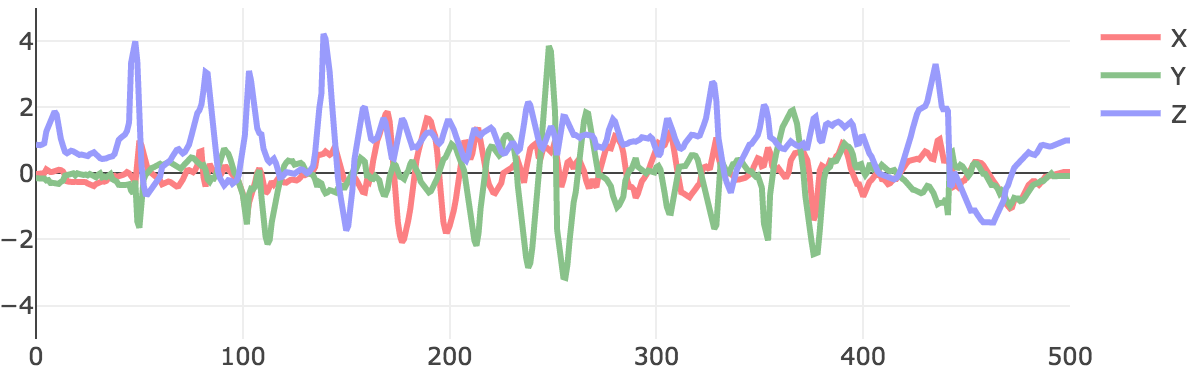
\includegraphics[width=15cm,keepaspectratio]{line_chart_2}
    \caption{line chart used to visualize sensor data in 2D and provide an interactive way to analyze the data}
    \label{fig:plotlylinechart}
\end{figure}

In GRAMOC the Plotly line chart was configured to hold three traces, one for each axis as shown in figure \vref{fig:plotlylinechart}. Plotly is designed to provide a convenient way to create interactive charts and not to provide high performance real-time charts, therefore it is used in the archive mode of GRAMOC and not in the real-time display.

\section{D3.js}
The name ``D3'' is an abbreviation of Data-Driven Documents, thats a very precise description of what this framework has to offer, namely the manipulation of documents based on data. The goal of D3 is not to visualize data on documents and at the same time be able to handle all the things around the objects as well as implementing every imaginable feature, it is build to be perfect at one thing: ``efficient manipulation of documents based on data'' as stated on their website \autocite{d3}. Since one of the key features of GRAMOC is real-time representation of the data that is provided by a sensor, this framework was chosen to be used within the real-time display. D3 has advantages as well as a few disadvantages, the probably biggest advantage is that this framework is very lightweight, this means there is only a minimal overhead and therefore it is very fast compared to other frameworks or libraries like \nameref{sec:Plotly}. A disadvantage of D3 would definitely be the lack of convenient high-level functions to create or modify objects. This means that a developer must write a lot of code to create for example, a simple line chart, in most high-level frameworks a developer just have to call one function to create a chart and another to add data to it. High-level functions are great to begin with, but to squeeze every last bit of performance out of the code, low-level functions are much better, also to understand what is happening behind the code low-level functions would be superior because the developer has to do nearly every step on his own and not just call a magic function that does a lot of processing on its own. Therefore the lack of high-level functions could be seen as an advantage, because programmers that use low-level functions instead of high-level functions often have more knowledge about how the system works and thats clearly a good thing.

\subsection{Line Chart}
In GRAMOC D3 was used to create a simple line chart to be able to visualize scientific sensor data in real-time. The chart is based on the line chart provided by Plotly, but with the distinction that the D3 chart can render the given data faster, and therefore sustain the real-time support of the application. The design should be similar to the Plotly line chart to maintain a uniform design within the application. The chart with example data is shown below in figure \vref{fig:d3linechart}.

\begin{figure}[H]
    \centering
    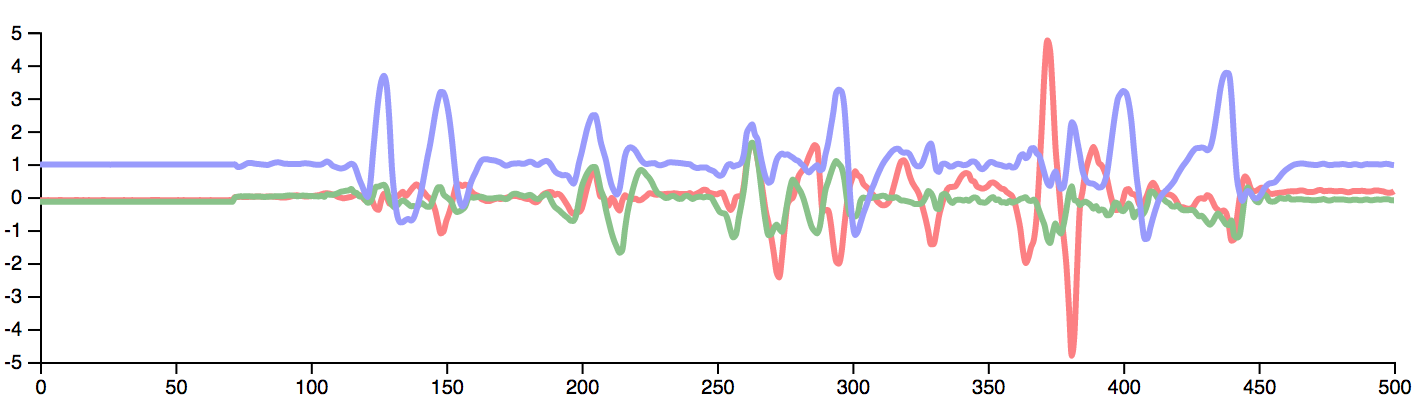
\includegraphics[width=15cm,keepaspectratio]{d3_line_chart}
    \caption{line chart used to visualize sensor data in 2D and be able to render in real-time}
    \label{fig:d3linechart}
\end{figure}

\section{Implementation}
As shown in figure \vref{fig:webserver-program-flow} the server asynchronously tries to connect with the UDP socket and starts listening for incoming connections on a specified port. The server keeps retrying to connect to the UDP socket until a connection is established. Without this connection no live data from the sensor can be forwarded to the web application. If a client connects on the before specified port the connection will be immediately upgraded to a socket connection and the web application will be served to the user. When the Webapp launches it will display the Home page, then the user can navigate to the 2D, the Archive or the About page, through the navigation bar at the top.

\subsection{2D Page}
If the user navigates to the 2D page, a line chart created with D3.js will be loaded. This chart consists of 3 traces, one for each axis of the sensor. The second chart displayed is a density chart created with HTML5 Canvas. This chart is represented by an ellipse, which is bent or stretched according to the received sensor data. Both these charts will be initialized and then the client emits a message to the server to start receiving the sensor data. This data will be used to update the charts accordingly. This page is responsible for visualizing the sensor data in real time and therefore its components are optimized to provide the necessary performance. The exact procedure is shown in figure \vref{fig:2d-page-flow}.

\begin{figure}[H]
    \centering
    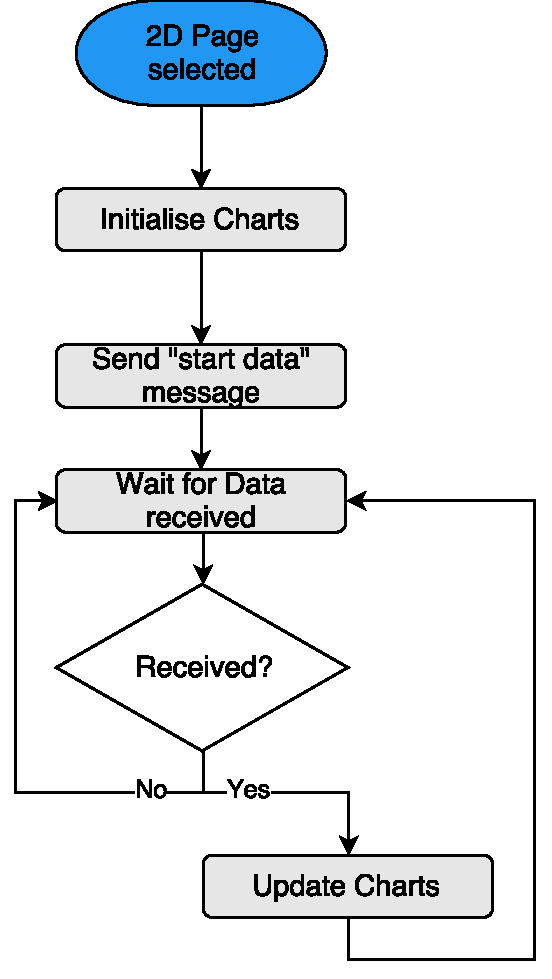
\includegraphics[width=5cm,keepaspectratio]{2d_page_flow}
    \caption{Flowchart of the procedure when 2D page is selected}
    \label{fig:2d-page-flow}
\end{figure}

\subsection{Archive Page}
The Archive page displays a line chart similar to the line chart on the 2D page, but with the focus on convenience rather than real-time performance. Therefore, Plotly is chosen to be used within this component. Along with the chart, a form will be available which is responsible to request the already recorded sensor data selected by the user. The execution flow of this component is depicted in figure \vref{fig:archive-page-flow}.

\begin{figure}[h]
    \centering
    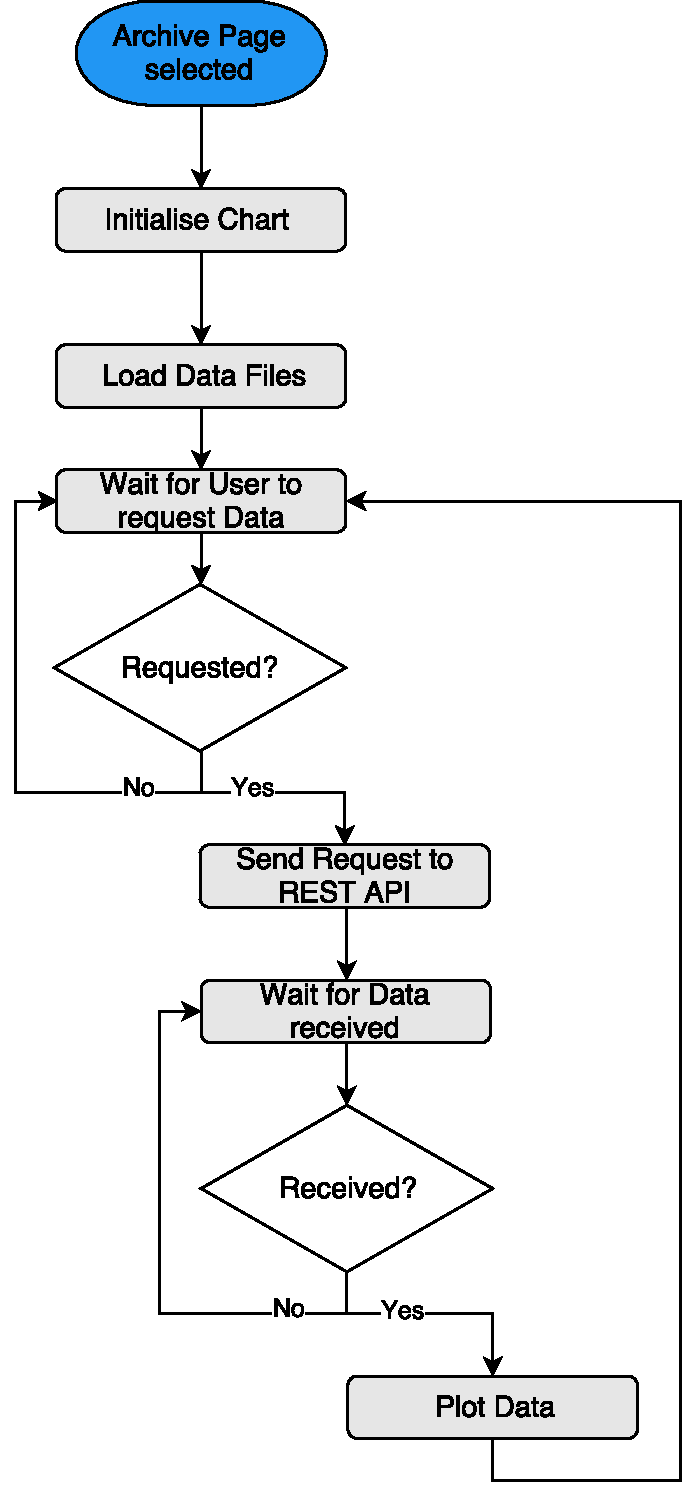
\includegraphics[width=7cm,keepaspectratio]{archive_page_flow}
    \caption{Flowchart of the procedure when Archive page is selected}
    \label{fig:archive-page-flow}
\end{figure}

\subsection{About Page}
The About page is simply a static page that displays a few informations about the project.

\begin{figure}[h]
    \centering
    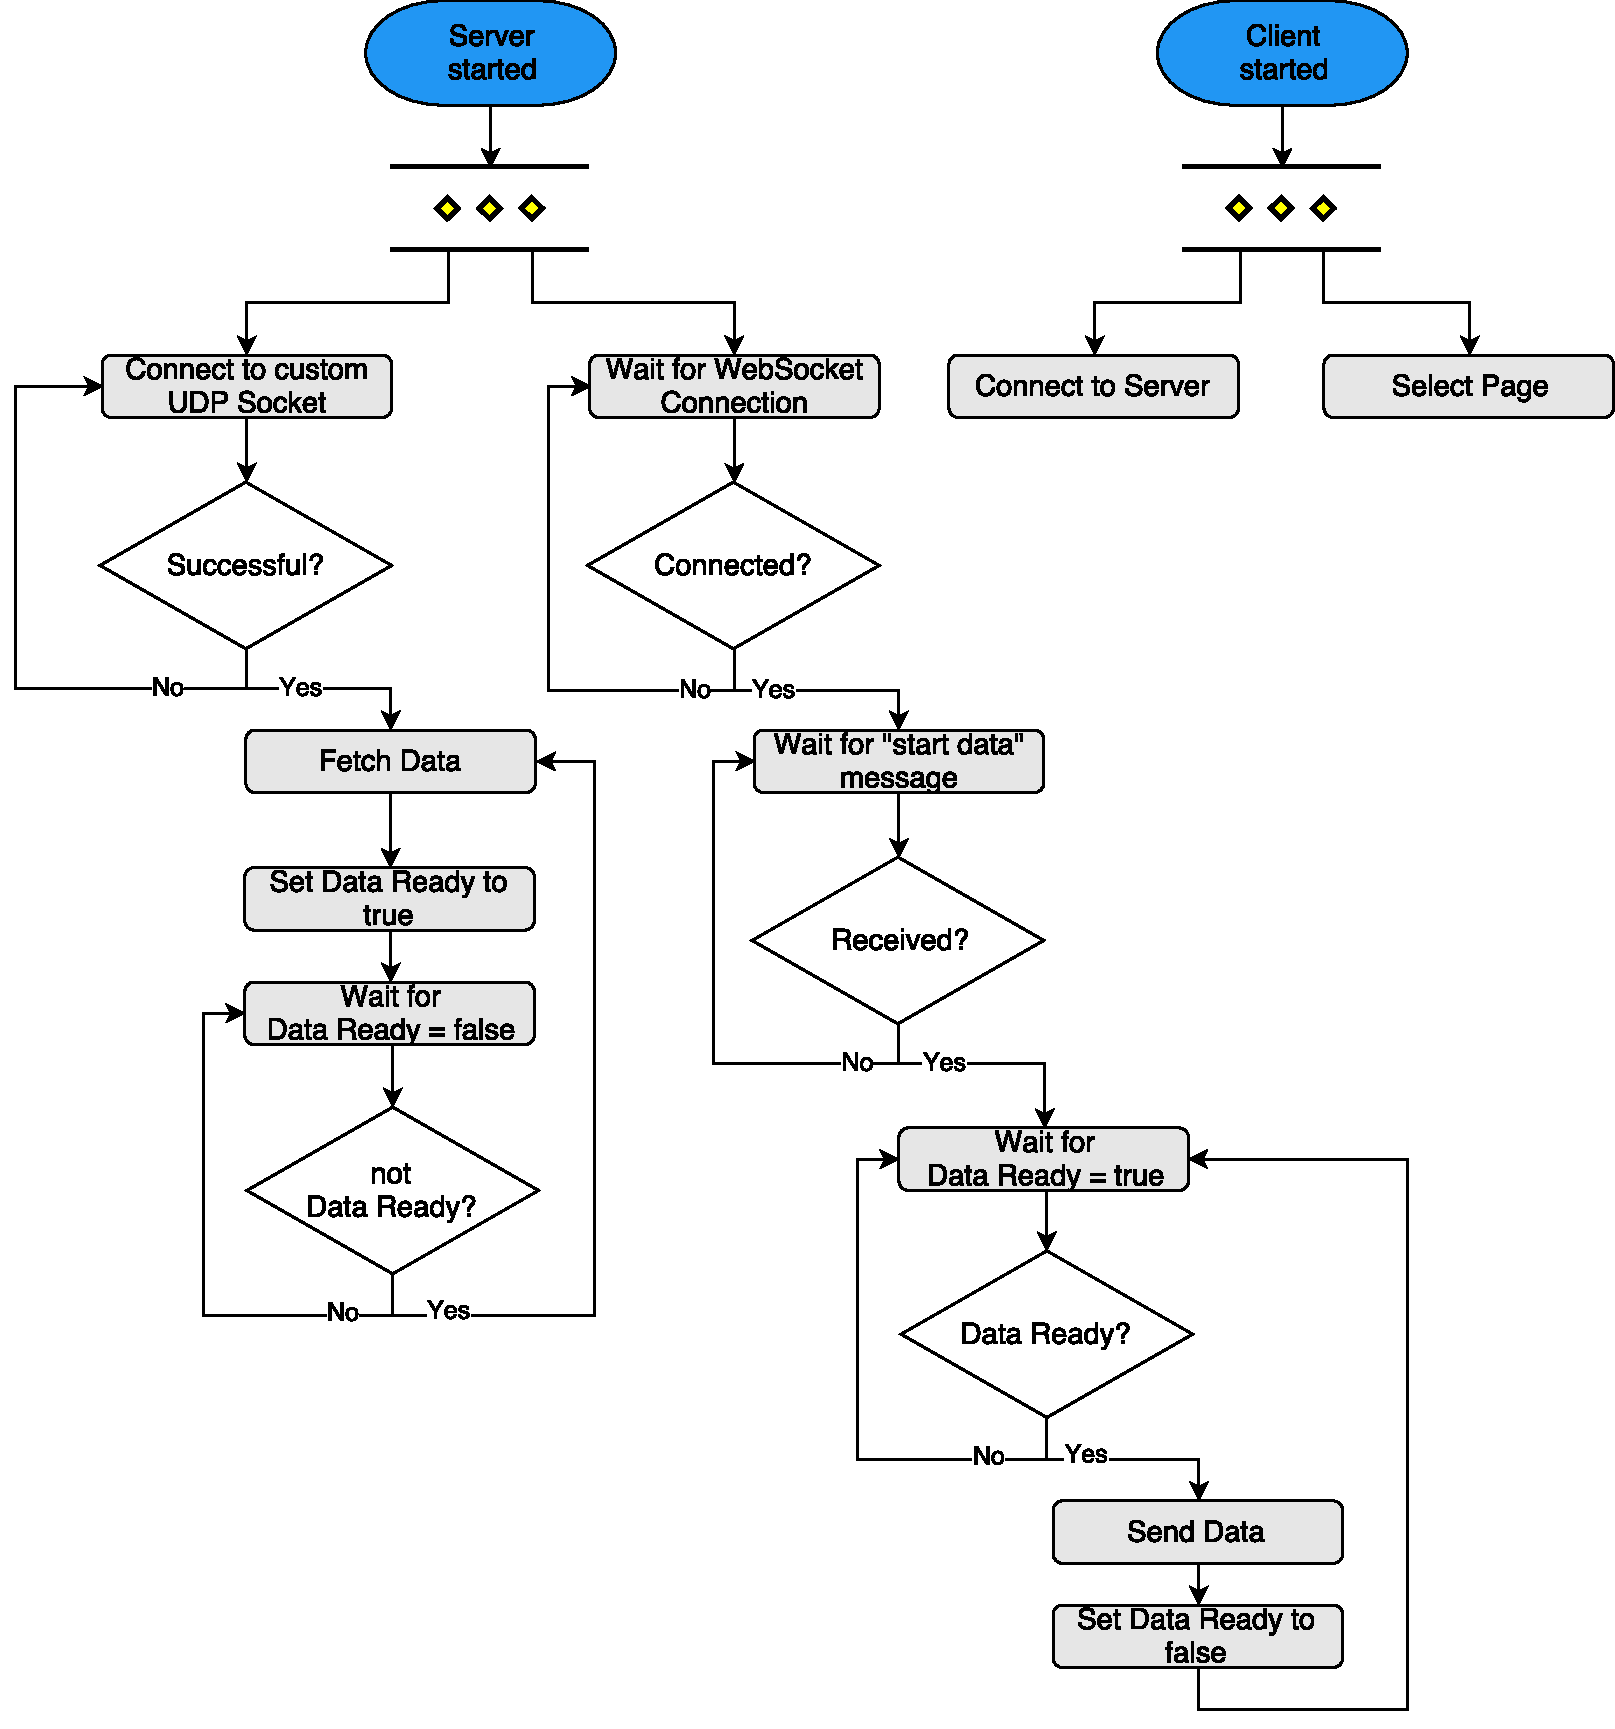
\includegraphics[width=15cm,keepaspectratio]{node_server_flow}
    \caption{Flowchart of web server and client program showing the procedure}
    \label{fig:webserver-program-flow}
\end{figure}
